\subsection{Trực quan hóa: Ánh xạ động}
Dữ liệu thị trường chứng khoán thay đổi linh hoạt trong ngày do giá thị trường liên tục được cập nhật trong phiên giao dịch. Vande Moere [436] đề xuất một cách thức trực quan hóa những dữ liệu như vậy bằng các chùm thông tin (\textit{flocking boids}). Thuật ngữ “boids” mượn từ sự mô phỏng của các loài chim trong đàn (các đối tượng chim = các boid). Để trực quan hóa giá thị trường chứng khoán, mỗi cổ phiếu được coi là một boid với vị trí ban đầu ngẫu nhiên trong không gian ba chiều. Khi có dữ liệu mới, các vị trí boid được cập nhật tự động theo một số quy tắc. Các quy tắc này thường được xây dựng để hướng tới các mục đích như: (i) tránh sự va chạm giữa các đối tượng di chuyển, (ii) đảm bảo tốc độ di chuyển các đối tượng trong cùng một chùm là giống nhau, (iii) các đối tượng có xu hướng di chuyển về phía trung tâm của đàn, và (iv) đảm bảo các đối tượng có độ tương đồng cao sẽ di chuyển gần nhau trong khi các đối tượng khác nhau sẽ di chuyển xa nhau. Cách thức biểu diễn trực quan hóa này có tính “động” đặc thù giúp thúc đẩy khả năng của người phân tích để nhận biết các xu hướng, mẫu hình (nếu có) khi các chùm di chuyển. Để làm được điều này, các đối tượng (boids) và đường đi của chúng phải được hiển thị dưới dạng các đường cong sinh động, như thể hiện ở Hình (\ref{fig:f7.13}) (hình bên trái). Ta cũng có thể nâng cấp cách biểu diễn trực quan 3D này bằng cách bao đóng các chùm bên trong các bề mặt ẩn, giúp người dùng có thể dễ dàng hơn trong việc nhận diện cấu trúc không gian của chùm (xem Hình (\ref{fig:f7.13}), bên phải). Các chùm có thể sẽ rất hữu ích trong việc khai phá, tìm kiếm các xu hướng, mẫu hình khác nhau trong bộ dữ liệu, chẳng hạn như sự tồn tại của các chùm dữ liệu, sự tách biệt của các chùm con khỏi chùm chính hoặc hành vi khác nhau của các đối tượng trong cùng một chùm.
\begin{figure}[H] % places figure environment here   
    \centering % Centers Graphic
    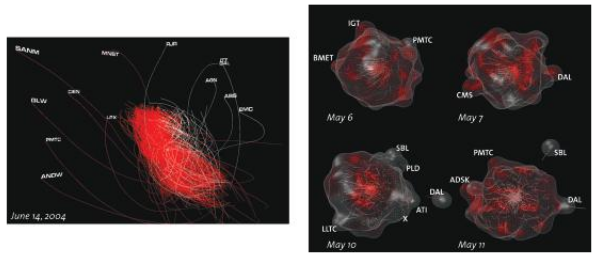
\includegraphics[width=0.8\textwidth]{assets/fig_7_13.png} 
    \caption{Chùm dữ liệu [436]. Dữ liệu thị trường chứng khoán được thể hiện dưới dạng các chùm di chuyển trong không gian ba chiều. Bên trái: các đối tượng tách khỏi chùm cho thấy giá cổ phiếu tương ứng có xu hướng vận động khác với phần lớn giá của các cố phiếu khác; bên phải: các bề mặt ẩn bao quanh các khối giúp người dùng nhận biết cấu trúc không gian của chùm.} % Creates caption underneath graph
    \label{fig:f7.13}
\end{figure}